\section{Hardware Implementation} \label{sec:implementation}
\vspace{-5pt}
%
In order to evaluate the performance and resiliency, we implements REMARK on an Intel 8051 based NVP as well as a hardware platform, \emph{NVnode}.
In this section, we first present the hardware platform in Sec.~\ref{sec:implHW}. 
Then, the improvement of the peripheral recovery and the overall performance are presented in Sec.~\ref{sec:implPeriRecover} and Sec.~\ref{sec:implOverall}, respectively. 

\subsection{Hardware Platform} \label{sec:implHW}
\vspace{-5pt}
%NVP
Fig.~\ref{fig:NVnode} shows a picture of NVP chip and NVnode platform.
The structure of NVnode is presented in Fig.~\ref{fig:ImpNVRF}.
NVnode contains a power supply system, an NVP with proposed REMARK modules and peripherals including ZigBee transceiver and sensors.
The energy storage is a $20\mu F$ capacitor which is charged between $1.2V$ and $5V$.
The total storage of the capacitor is $212\mu J$ while the energy efficiency is $90\%$.

% NVP
The parameters of the proposed NVP are listed in Table.~\ref{tab:NVnodePara}.
This NVP is designed based on Intel 8051 ISA. 
It contains a $256B$ register file using NVFF, a $32KB$ FeRAM data memory, a B/R Manager and an NVRF module to enable REMARK.

% NVRF
As shown in Fig.~\ref{fig:ImpNVRF}, NVRF realizes the functionality of PSRs and PRM, which enable efficient and reliable peripheral configuration and restart operations.
NVRF contains a $32B$ register file, an RF controller, and an SPI interface.
The register file stores the state of the wireless transceiver.
The RF controller can reconfigure the transceiver and restart the data transmission task automatically and efficiently after power failure.
The SPI interface is used to mount to SPI bus, which also connect to a ZigBee transceiver and several sensors.

%
\begin{figure}[t]
    \centering
    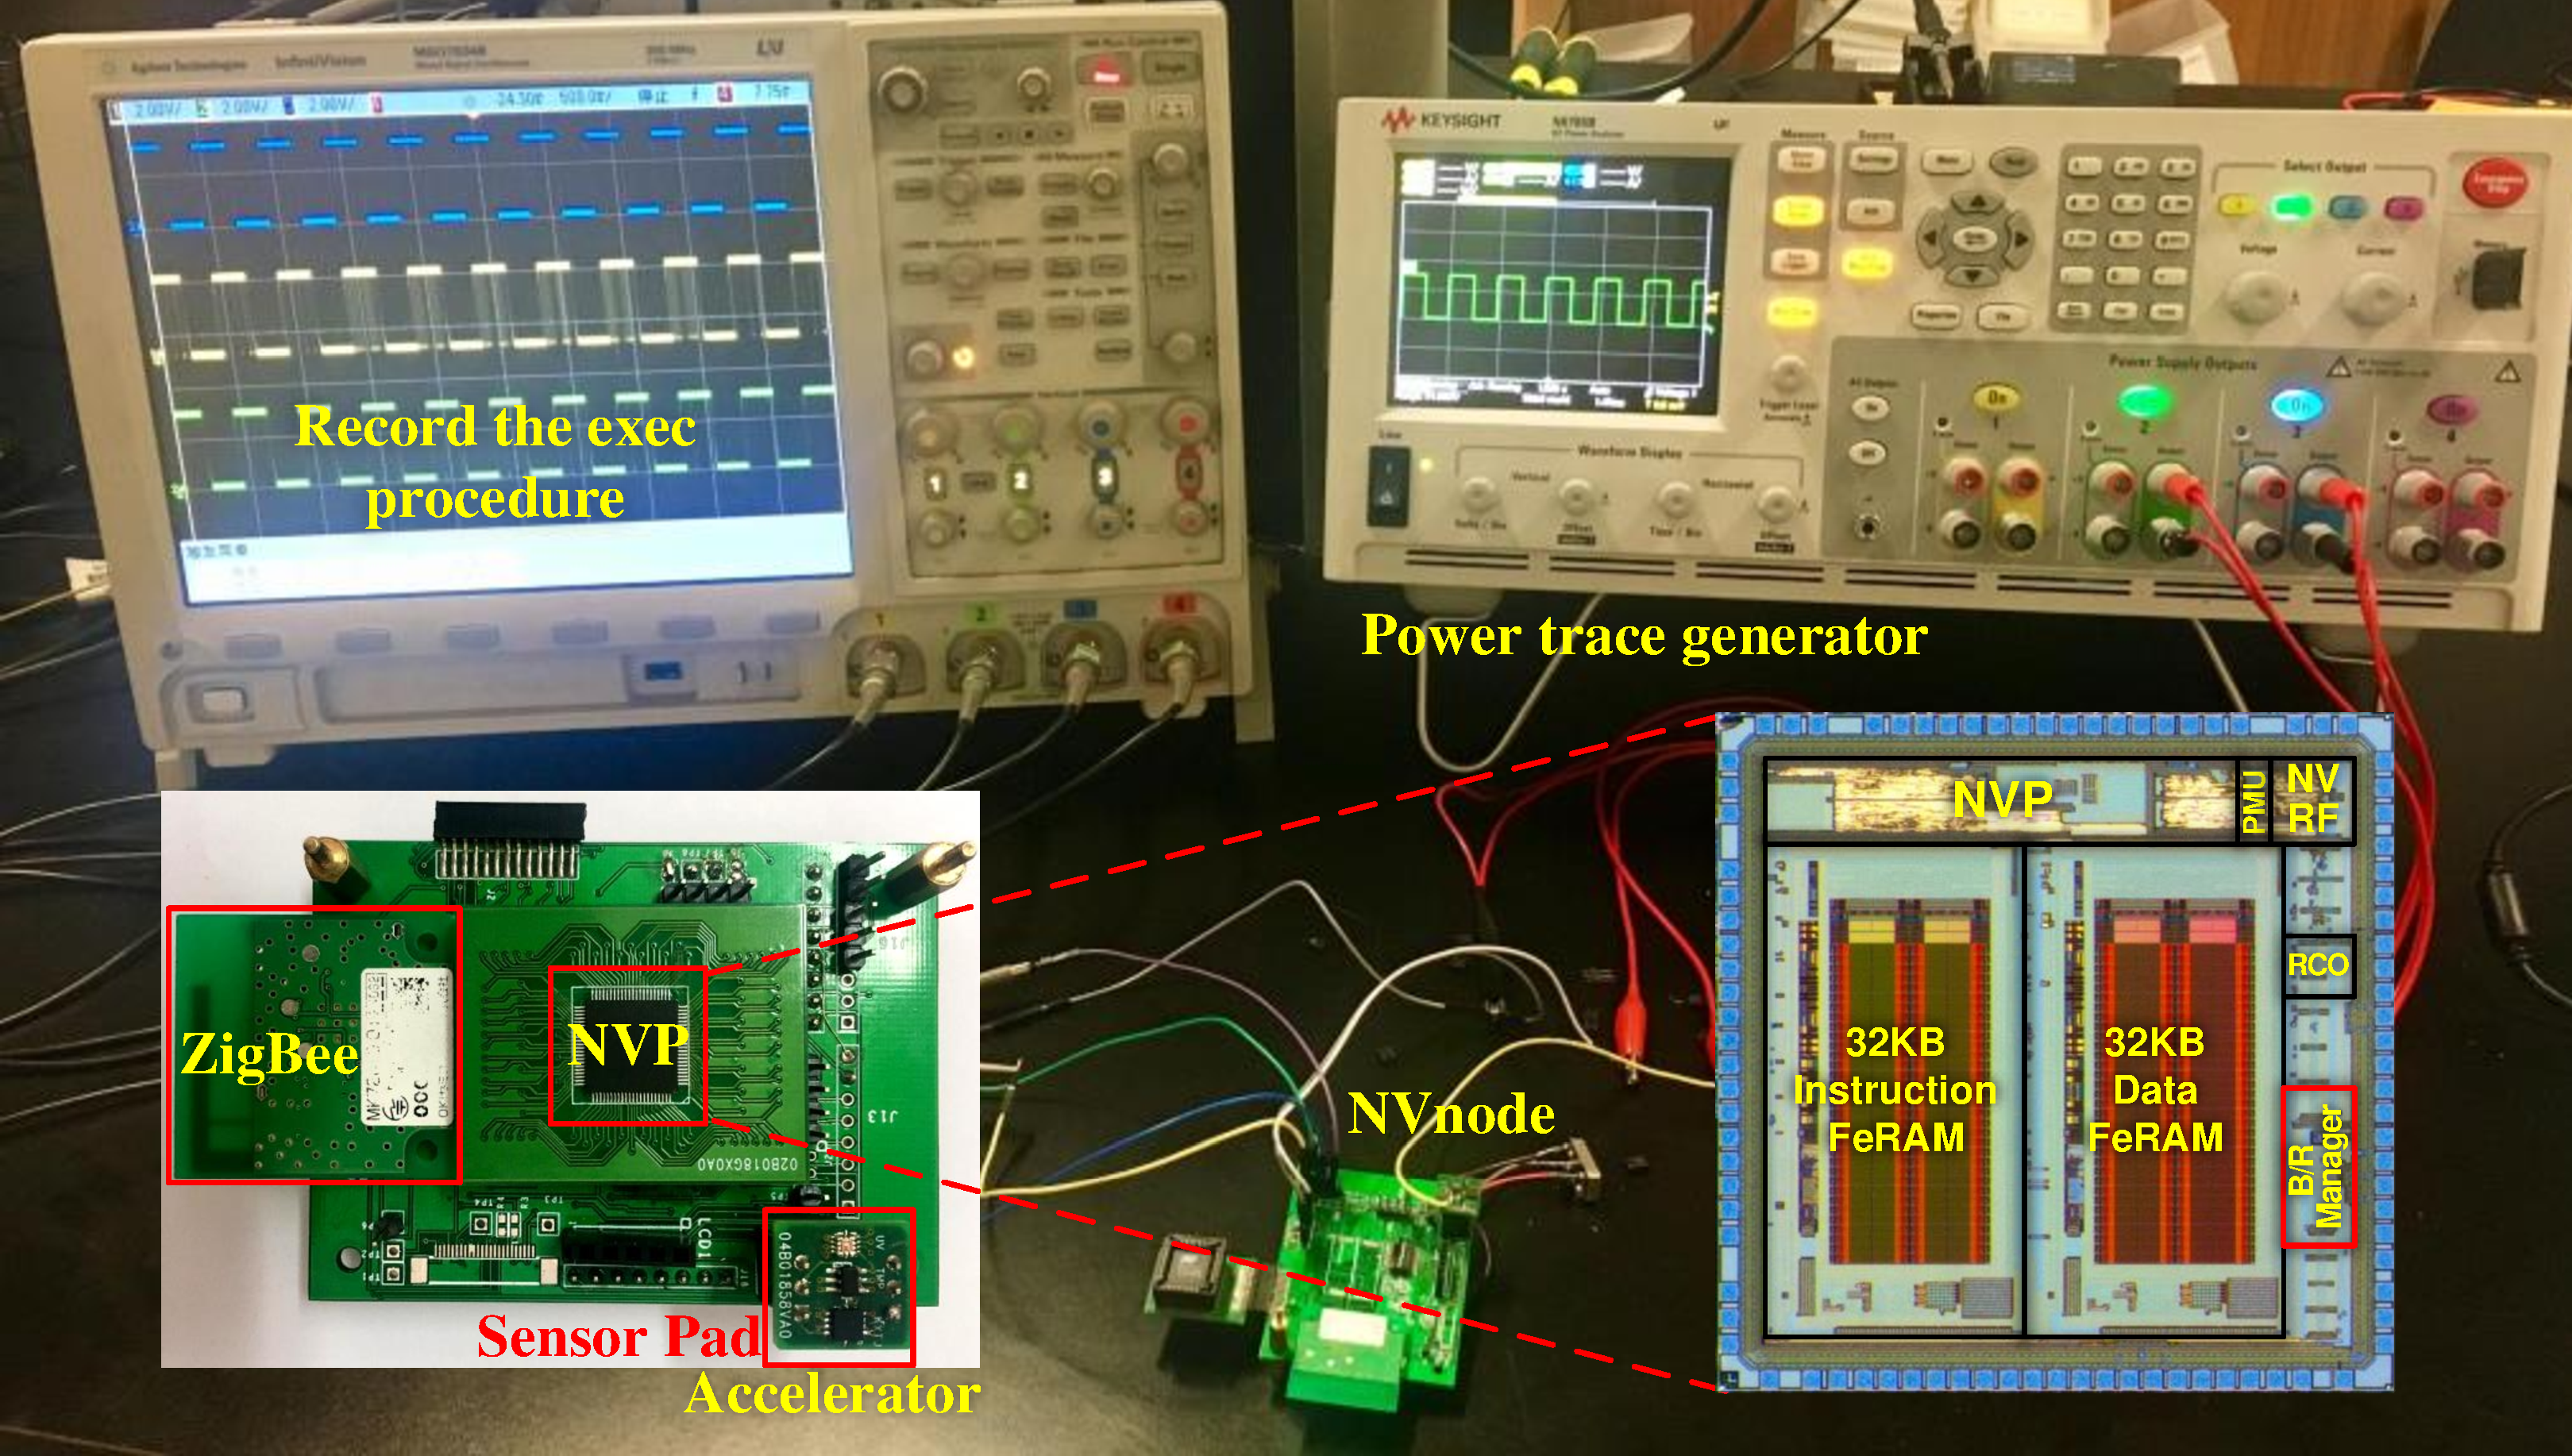
\includegraphics[width=0.48\textwidth]{Fig11_NVnode.pdf}
    \vspace{-10pt}
    \caption{The hardware platform, NVnode. REMARK is implemented with the B/R manager and the NVRF controller in an 8051 NVP chip under $0.13\mu m$ technology.}
    \vspace{-5pt}
    \label{fig:NVnode}
\end{figure}

\begin{figure}[htpb]
    \centering
    \vspace{-0pt}
    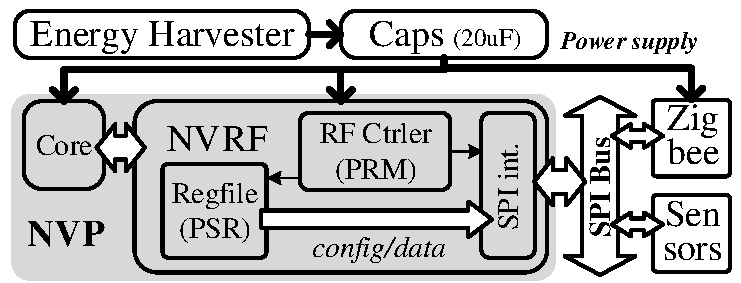
\includegraphics[width=0.4\textwidth]{Fig11_ImpNVRF.pdf}
    \vspace{-2pt}
    \caption{The structure of NVnode. The energy storage is $20\mu F$. NVRF implements the functionality of PSRs and PRM to accelerate the peripheral recovery.}
    \vspace{-5pt}
    \label{fig:ImpNVRF}
\end{figure}

\begin{table}[t]
\begin{center}
\vspace{-0pt}
\caption{The parameters of NVP.} \label{tab:NVnodePara}
\vspace{-5pt}
\Fsize{8}
\renewcommand{\arraystretch}{1.5}
%\setlength{\tabcolsep}{1pt}
\begin{tabular}{Ic|cIc|cI}
    \Xhline{1.2pt}
    Parameter                        & Value                    & Parameter                    & Value        \\
    \Xhline{1pt}
    Process Technology        & $0.13\mu m$         & Clock frequency           & $1MHz$        \\
    %\Xhline{1pt}
    %TMP Sensor                    & TMP100               & RF Module                   & ML7266    \\
    \Xhline{1pt}
    Backup Time                  & $5\mu s$               & Restore Time                & $3\mu s$   \\
    \Xhline{1.2pt}
\end{tabular}
\vspace{-15pt}
\end{center}
\end{table} 

\subsection{Device Recovery Improvement of REMARK} \label{sec:implPeriRecover}
\vspace{-5pt}
%
To show the effectiveness of REMARK, this subsection first shows the overhead reduction of a single transceiver recovery. 
Then, it shows the efficiency improvement when there are multiple peripheral devices. 
REMARK is compared with the traditional single device recovery strategies, such as QuickRecall~\cite{jayakumar2014quickrecall}. 
Since the hardware platform utilizes NVP, a single device rollback strategy (SDRB) is designed based on QuickRecall in NVnode for comparison purposes.
SDRB restarts the peripheral by the processor executing configuration and restart functions.

Fig.~\ref{fig:ImpCompare} (a) compares the transceiver recover time between the hardware NVRF and the software recover procedure, SDRB.
After power failure, NVRF automatically configures and restarts the transceiver in $1.22ms$.
During this procedure, NVRF first restores the register file in $9 \mu s$, and then performs the configuration and restart operation in $0.91ms$ and $0.31ms$, respectively. 
SDRB performs the recovery with three steps.
Firstly, the processor recovers the configurations and the data of the transceiver in the NVFFs in $9\mu s$.
Then, the transceiver is reset and configured via SPI interfaces in $25.3ms$.
Finally, the transmission operation is restarted in $7.7ms$.
The total overhead of software recovery is 33ms.
Thus, REMARK accelerates the process by $27.0\times$. 

Fig.~\ref{fig:ImpCompare} (b) shows the comparison between the multi-device checkpointing strategy in REMARK and the rollback strategy in SDRB.
From the figure, we can see that, REMARK places checkpoints of NVP and the transceiver individually and realizes parallel recovery with the help of NVRF.
The distributed rollback strategy for multi-device TPC recovers the peripherals and the processor in parallel.
The total recovery overhead of REMARK equals to the largest recovery overhead of each device, which is smaller than recovering all the devices in serial.
Moreover, the \emph{`init-used'} strategy allows REMARK only to recover a peripheral when it is invoked, while SDRB suffers large re-configuration overhead adopting the \emph{`init-all'} strategy.
In addition, SDRB also introduces processor rollbacks, whose overhead is related to the power failure position.
With these factors, REMARK accelerates the peripheral recovery procedure by $34.1\times$ than SDRB in this case.

%
\begin{figure*}[htpb]
    \centering
    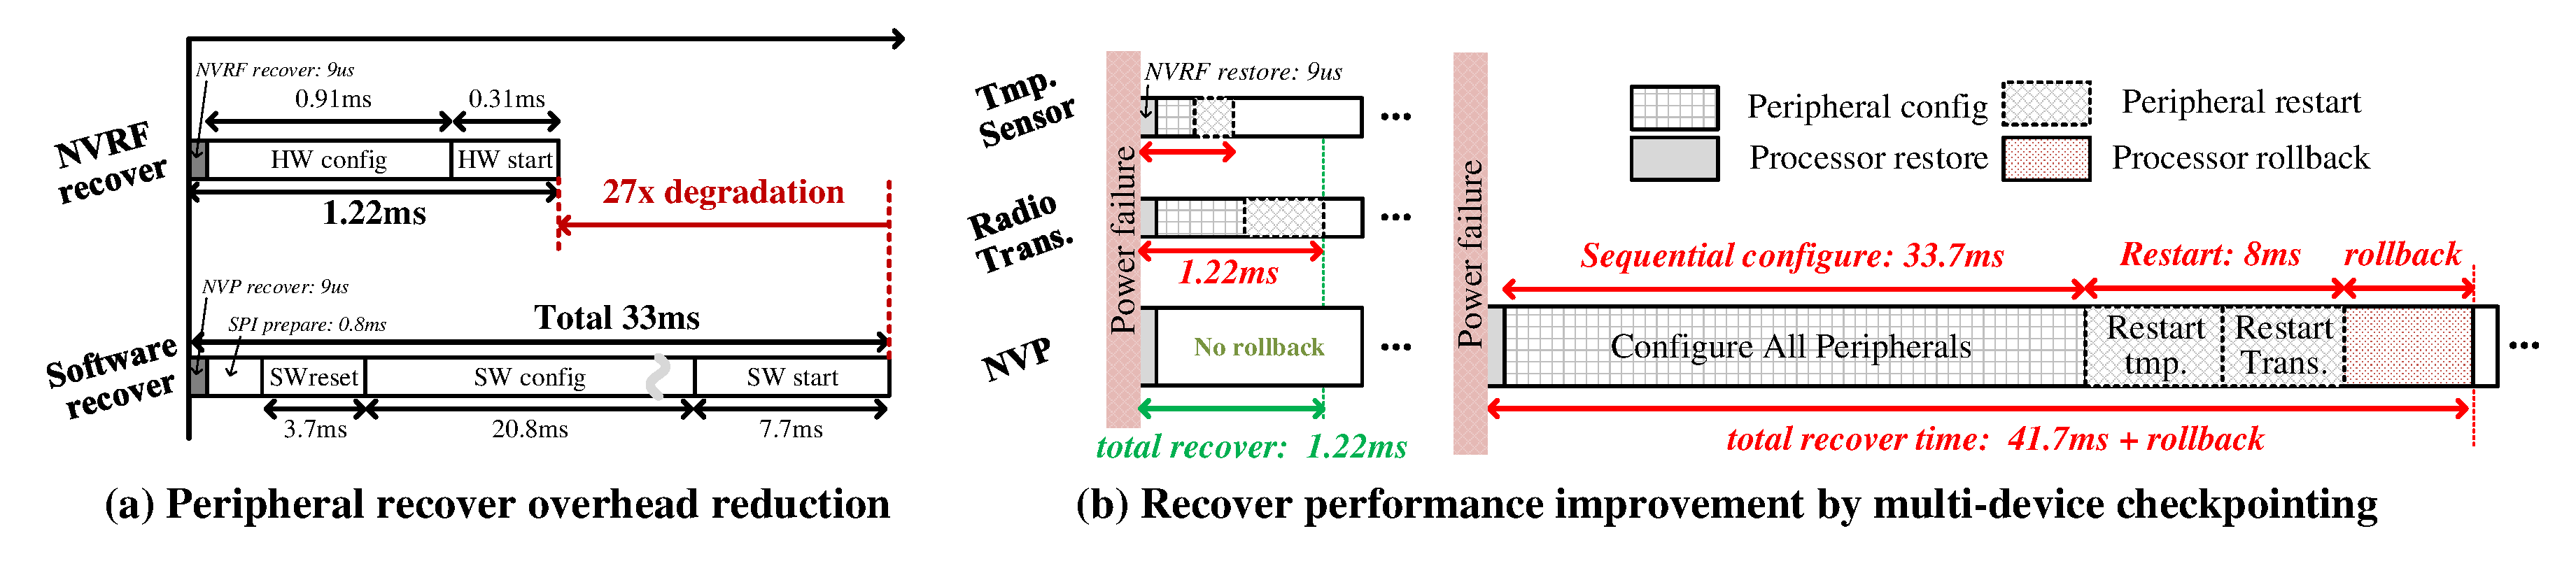
\includegraphics[width=1\textwidth]{Fig12_ImpCompare.pdf}
    \vspace{-25pt}
    \caption{Recover overhead and task completeness comparison between REMARK and SDRB.}
    %\vspace{-5pt}
    \label{fig:ImpCompare}
\end{figure*}

\subsection{Overall Performance Evaluation} \label{sec:implOverall}
\vspace{-5pt}
%
The improvement in recovery performance leads to better overall system performance. 
A \emph{`bridge-monitoring'} application, a pure transmission application, and a pure sensing application are used to evaluate the overall performance improvement.
\emph{`bridge-monitoring'} is a data collecting application which contains both sensing and transmission tasks. 
These tasks are repeated periodically.
The work flow of \emph{`bridge-monitoring'} is shown in Fig.~\ref{fig:ImpOverall} (a).
The power trace is a Wi-Fi power profile, whose average power is $93.3\mu W$.
NVnode starts to work, when the capacitor is charged to $5V$.
The system fails and the capacitor gets recharged when the voltage of capacitor falls below $1.2V$.

The benchmarks are executed for $2$ minutes with REMARK and SDRB.
Fig.~\ref{fig:ImpOverall} (b) compares the task completion efficiency.
For the benchmarks with pure transmission and sensing tasks, REMARK achieves $5.7\times$ and $5.6\times$ efficiency improvements.
For the ‘bridgemonitoring’ benchmark, REMARK completes $13\times$ more data collection and transmission tasks than SDRB.
This is because the latter contains more peripherals where the performance of SDRB significantly deteriorates.
Due to the improvement in task completion efficiency, the energy consumption is also reduced accordingly. 

\begin{figure}[t]
    \centering
    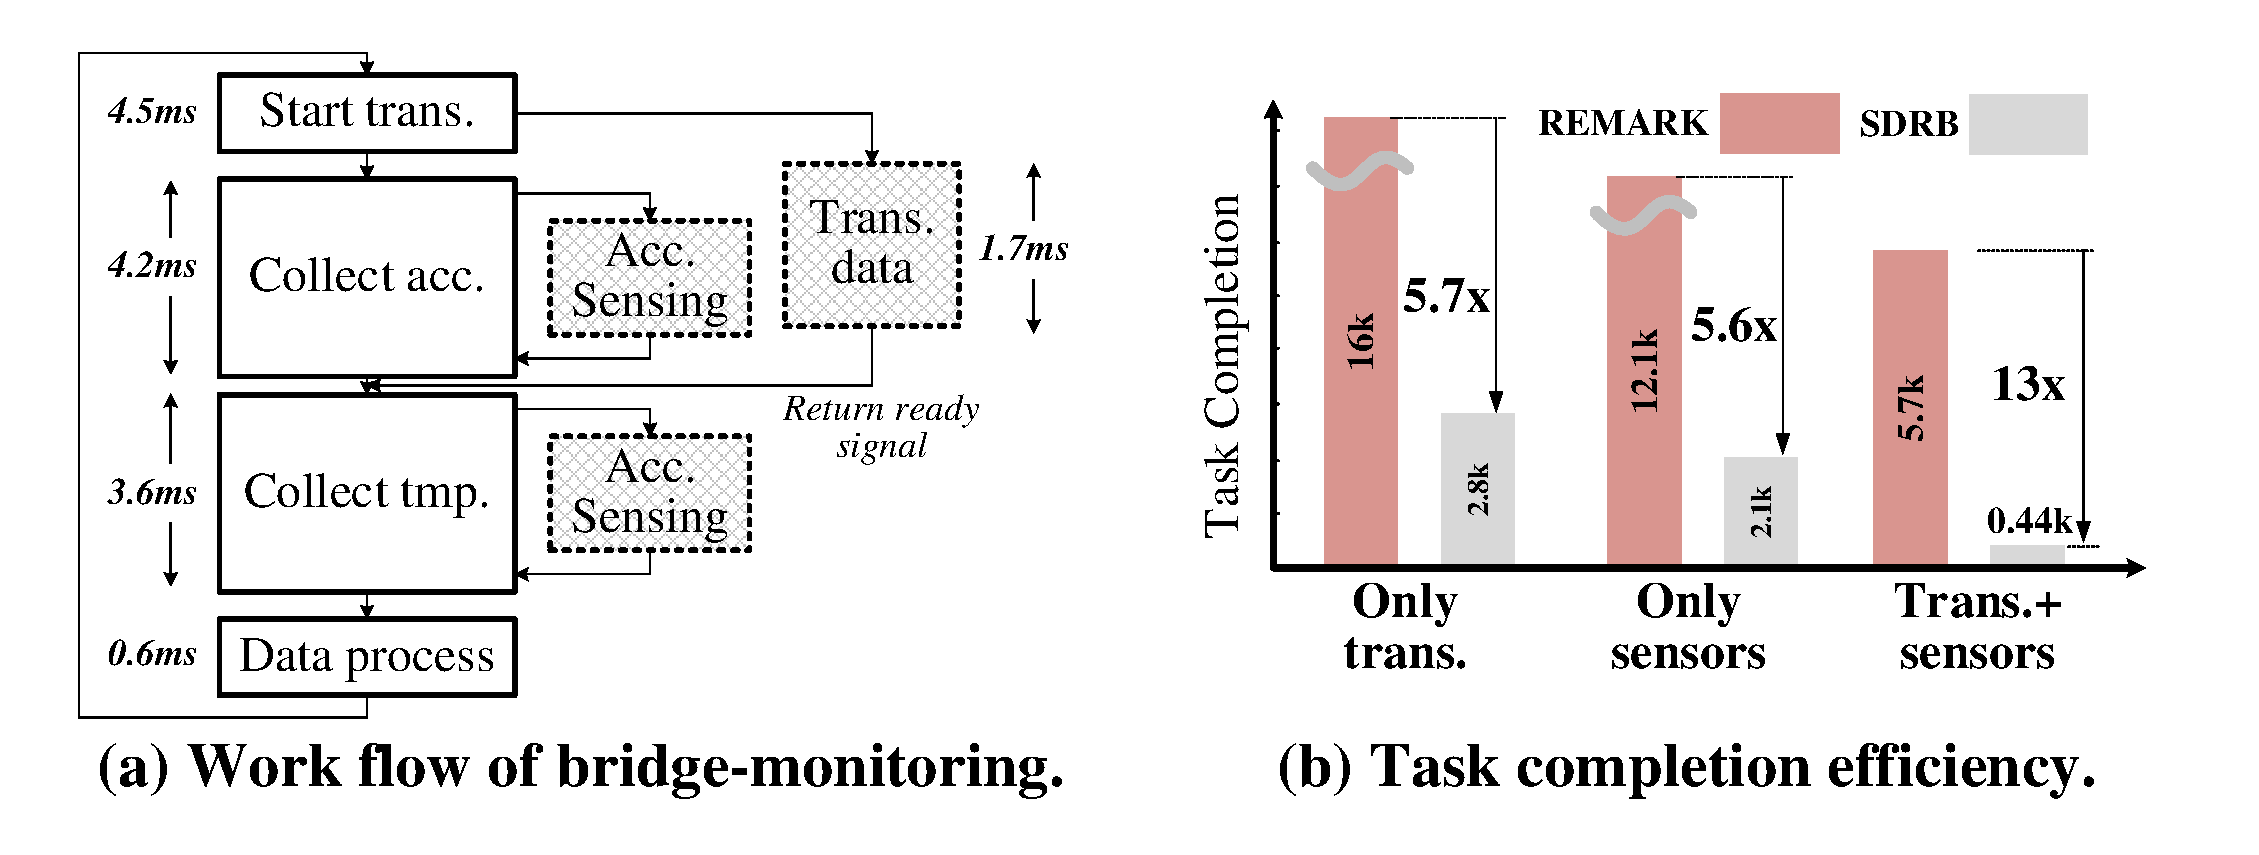
\includegraphics[width=0.5\textwidth]{Fig12_ImpOverall.pdf}
    \vspace{-20pt}
    \caption{\emph{bridge-monitoring} application and task completeness comparison between REMARK and SDRB.}
    \vspace{-5pt}
    \label{fig:ImpOverall}
    \vspace{-0pt}
\end{figure}

\begin{comment}
%
\begin{figure}[t]
    \centering
    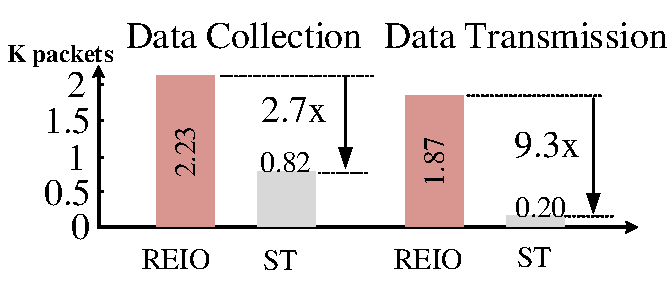
\includegraphics[width=0.3\textwidth]{Fig12_ImpRecover.pdf}
    \vspace{-10pt}
    \caption{Performance comparison of REMARK and REMARK by executing \emph{bridge-monitoring} for $2$ minutes on NVnode.}
    \label{fig:ImpRecoverEvaluate}
    \vspace{-0pt}
\end{figure}

\begin{comment}
{To decouple the effect of outage rates, Fig.}~\ref{fig:ImpRecoverEvaluate}{ (a) shows an example of a typical recover procedure after one power failure, where REMARK reduces the recovery overhead by 61.8\%.}
%Fig.~\ref{fig:ImpRecoverEvaluate}{ (c) shows the overhead breakdown of REMARK and QuickRecall. REMARK improves the validate execution time from total overheads.}
 
%\noindent$\bullet$
\textbf{Re-initialization overhead} 
        Compared with the \emph{`init-all'} strategy in QuickRecall, REMARK reduces the re-initialization overhead from 55\% to 11\% with the \emph{`init-used'} strategy.

\textbf{B/R overhead} 
        B/R overhead represents the backup/restore overhead. Using hardware B/R functions, REMARK incurs negligible B/R time overhead.
     
\textbf{Rollback overhead} 
        The rollback overhead is a random scaled overhead which depends on the position where power failure disrupts the program. REMARK is able to complete more tasks with comparable rollback overheads of QuickRecall.


In conclusion, \emph{REMARK guarantees the reliability of I/O and peripheral operations, and the data transmission/collection completeness is improved by $9.3\times$/$2.7\times$  compared with the existing state-of-the-art software recovery strategies}.

%
\begin{figure}[t]
    \centering
    \includegraphics[width=0.5\textwidth]{Fig13_ImpOverheadDeadlock.pdf}
    \vspace{-20pt}
    \caption{{Overhead and resilience analysis. (a) the overhead of wrapper code. (b) a micro case study of the worst case when the outage rate is too high. (c) a sweep analysis of recovery overhead with power failure rates.}}
    \label{fig:ImpOverheadDeadlock}
    \vspace{5}
\end{figure}
\end{comment}